\begin{flushleft}
Per confrontare i risultati tra il nostro procedimento di calcolo di $k_{\infty}(A)$ e quello della function cond di MatLab, abbiamo scritto il seguente script:
\lstinputlisting[language=Matlab]{cap_3/es15/es15.m}
\label{es315}
Che restituisce come output:
\begin{figure}[h]
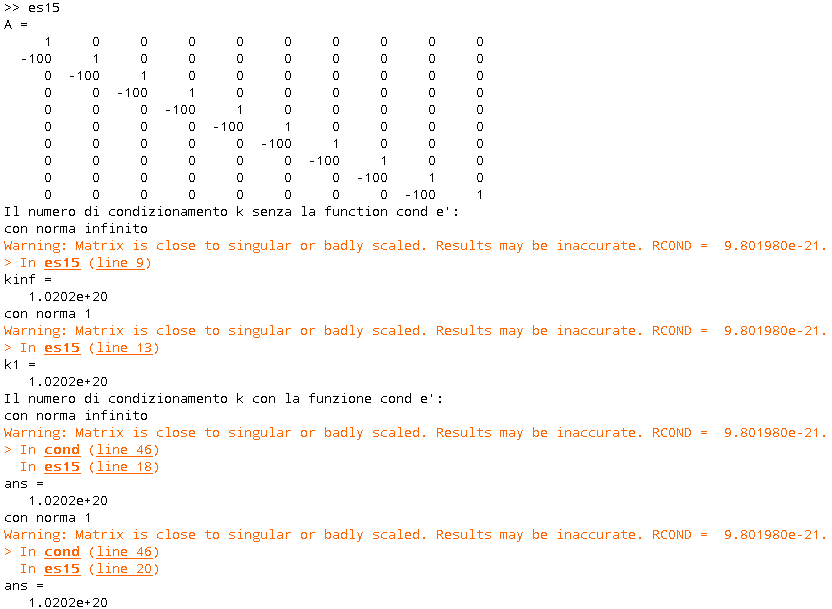
\includegraphics[left, width=250px]{cap_3/es15/es315}
\end{figure}
\newline \\
Dall'output possiamo vedere che $k_{\infty}$ che per $k_1$ risultano uguali con valore pari a $1.0202\cdot 10^{20}$. Inoltre sia cond che inv restituiscono come warning:
\begin{figure}[h]

\includegraphics[left, width=250px]{cap_3/es15/es315e}
\end{figure}
\newline \\
che significa che il problema dell'inversione della matrice può non essere accurato perchè la matrice è mal condizionata.
Dobbiamo ora dimostrare che $k_{\infty}(A)=k_{1}(A)$, cioè:
\[
\Big|\Big|A\Big|\Big|_{\infty} \cdot \Big|\Big|A^{-1}\Big|\Big|_{\infty} = \Big|\Big|A\Big|\Big|_{1} \cdot \Big|\Big|A^{-1}\Big|\Big|_{1}
\]
Possiamo calcolare $\Big|\Big|A\Big|\Big|_{\infty}$ che ovviamente sarà pari a 101 dato che gli unici 2 valori ottenuti dalla somma dei valori assoluti degli elementi riga della matrice sono 1 e 101, da cui possiamo affermare che il massimo tra i due è 101. Per $\Big|\Big|A\Big|\Big|_{1}$ i valori delle somme dei valori assoluti degli elementi colonna della matrice sono 1 e 101, come per la precedente norma otteniamo quindi il valore massimo 101. Sappiamo quindi che $\Big|\Big|A\Big|\Big|_{\infty}=\Big|\Big|A\Big|\Big|_{1}$. Rimane da dimostrare che $\Big|\Big|A^{-1}\Big|\Big|_{\infty} = \Big|\Big|A^{-1}\Big|\Big|_{1}$. Per farlo possiamo andare a calcolare la matrice inversa $A^{-1} = \frac{1}{\text{det}(A)}A^{*}$, in cui $A^*$ è la matrice aggiunta calcolata come segue:
\newpage
\[
a^*_{1,1} = \text{det}\big|A_{1,1}\big| = 1 = a^*_{2,2} = a^*_{3,3} = ... = a^*_{10,10}
\]
\[
a^*_{2,1} = \text{det}\big|A_{1,2}\big| = 10^2 = a^*_{3,2} = a^*_{4,3} = ... = a^*_{10,9}
\]
\[
a^*_{3,1} = \text{det}\big|A_{1,3}\big| = 10^4 = a^*_{4,2} = a^*_{5,3} = ... = a^*_{10,8}
\]
\[
.
\]
\[
.
\]
\[
.
\]
\[
a^*_{10,1} = \text{det}\big|A_{1,10}\big| = 10^{18} 
\]
\[
a^*_{1,2} = \text{det}\big|A_{2,1}\big| = 0 = a^*_{1,3} = ... = a^*_{1,10}
\]
(Abbiamo usato la notazione $A_{n,m}$ per la matrice che si ottiene a partire da A eliminando la riga n e la colonna m). Per i valori al di sopra della diagonale possiamo dire che sono in valore assoluto $<<1$. Dato che $\text{det}(A)=1$ allora $A^{-1} = A^*$:
\[
A^{-1}=\begin{bmatrix}
1&0&0&0&0&0&0&0&0&0\\
10^2&1&.&.&.&.&.&.&.&.\\
10^4&10^2&1&.&.&.&.&.&.&.\\
10^6&10^4&10^2&1&.&.&.&.&.&.\\
10^8&10^6&10^4&10^2&1&.&.&.&.&.\\
10^{10}&10^8&10^6&10^4&10^2&1&.&.&.&.\\
10^{12}&10^{10}&10^8&10^6&10^4&10^2&1&.&.&.\\
10^{14}&10^{12}&10^{10}&10^8&10^6&10^4&10^2&1&.&.\\
10^{16}&10^{14}&10^{12}&10^{10}&10^8&10^6&10^4&10^2&1&.\\
10^{18}&10^{16}&10^{14}&10^{12}&10^{10}&10^8&10^6&10^4&10^2&1\\
\end{bmatrix}
\]
Notiamo che la somma dei valori della riga 10 e della colonna 1 della matrice inversa sono identici, inoltre sono anche i valori ottenuti effettuando $\Big|\Big|A^{-1}\Big|\Big|_{\infty}$ e $\Big|\Big|A^{-1}\Big|\Big|_{1}$. Possiamo quindi affermare che $\Big|\Big|A^{-1}\Big|\Big|_{\infty} = \Big|\Big|A^{-1}\Big|\Big|_{1}$.
\end{flushleft}